\section{Pickup}
\label{pickup-project}

Electric guitars uses pickups consisted by magnets wrapped in thin  copper wire. The
working principle is based on the variation of magnetic field, created by the string
vibration. The vibration frequency of the string induces an electric signal on the output of the pickup \cite{pickup-work}
\cite{faraday-law}.

The designed pickup used the following main components:

{\begin{itemize}
  \item Base to assembly the set up magnet+coil
  \item 6 magnets
  \item Copper wire to wrap the magnets
  \item Cover to attach the set up on the guitar
\end{itemize}}

After some studies it was decided to build the pickup base using a 3D printer, due the
availability and reduced cost of this project. The model is showed on \autoref{3D-project}
and was projected using the AutoCAD software.

\begin{figure}[!htpb]
\centering
\caption{3D pickup base project}
\label{3D-project}
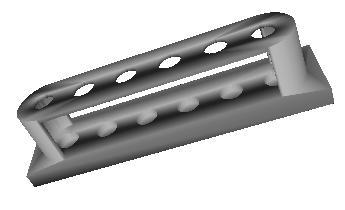
\includegraphics[scale=0.5]{images/pickup}
\legend{Source: Authors}
\end{figure}

There was two materials to print the model, \textit{PLA} (Polylatic Acid) \cite{3d-materials}
and \textit{ABS} (Acrylonitrile Butadiene Styrene) \cite{3d-materials}. It was decided to print
the model on PLA because it attends the requisites of robustness of the project, is
faster to print and have a lower cost when compared to the other material.

With pickup base ready it was assembled the coils around the guitar \autoref{magnets}.
It was performed some tests and it was chosen to use the 0.5mm diameter wire on the project,
giving 500 turns on each magnet to reach a minimal workable voltage value.

\begin{figure}[!htpb]
\centering
\caption{Magnets used on the project}
\label{magnets}
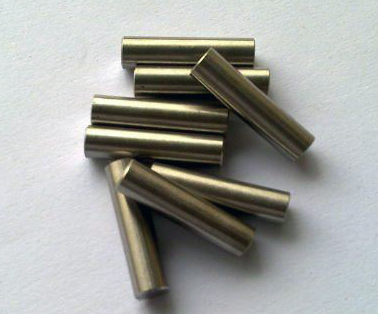
\includegraphics[scale=0.2]{images/magnets}
\legend{Source: \citeonline{pickup-magnets}}
\end{figure}
